% questions.tex —— 2007 年·普通高等学校招生考试·安徽卷·文科 · 题目内容片段（无答案）
% 由 tools/generate_projects.py 依来源总账自 2007/2007_数学真题_安徽文_试题.md 生成，勿手改（改源 MD 后重跑）


状态：needs-review；依固定候选 PDF 两页（印刷页 349–350）三栏图像以 300 dpi 渲染逐题核验，图形已矢量重绘，正式构建与逐页验收待完成。源未列各题分值，不补分值。

\gkpart{一、选择题}

\begin{question}
\gkti{1}若 $A=\{x\mid x^2=1\}$，$B=\{x\mid x^2-2x-3=0\}$，则 $A\cap B=$（　）

（A）$\{3\}$

（B）$\{1\}$

（C）$\varnothing$

（D）$\{-1\}$

\end{question}
\begin{question}
\gkti{2}椭圆 $x^2+4y^2=1$ 的离心率为（　）

（A）$\dfrac{\sqrt3}{2}$

（B）$\dfrac34$

（C）$\dfrac{\sqrt2}{2}$

（D）$\dfrac23$

\end{question}
\begin{question}
\gkti{3}等差数列 $\{a_n\}$ 的前 $n$ 项和为 $S_n$。若 $a_2=1$，$a_3=3$，$S_4=$（　）

（A）$12$

（B）$10$

（C）$8$

（D）$6$

\end{question}
\begin{question}
\gkti{4}下列函数中，反函数是其自身的函数为（　）

（A）$f(x)=x^2$，$x\in[0,+\infty)$

（B）$f(x)=x^3$，$x\in(-\infty,+\infty)$

（C）$f(x)=\mathrm e^x$，$x\in(-\infty,+\infty)$

（D）$f(x)=\dfrac1x$，$x\in(0,+\infty)$

\end{question}
\begin{question}
\gkti{5}若圆 $x^2+y^2-2x-4y=0$ 的圆心到直线 $x-y+a=0$ 的距离为 $\dfrac{\sqrt2}{2}$，则 $a$ 的值为（　）

（A）$-2$ 或 $2$

（B）$\dfrac12$ 或 $\dfrac32$

（C）$2$ 或 $0$

（D）$-2$ 或 $0$

\end{question}
\begin{question}
\gkti{6}设 $l,m,n$ 均为直线，其中 $m,n$ 在平面 $\alpha$ 内，则「$l\perp\alpha$」是「$l\perp m$ 且 $l\perp n$」的（　）

（A）充分不必要条件

（B）必要不充分条件

（C）充分必要条件

（D）既不充分也不必要条件

\Needspace{0.4\textheight}
\end{question}
\begin{question}
\gkti{7}图中的图象所表示的函数的解析式为（　）
\nopagebreak[4]
\begin{center}% 2007 年安徽卷文科第 7 题：定义在 [0,2] 上的折线图象，x=0 与 x=2 处为 0，
%   x=1 处为 3/2，两侧各为直线段。
% 来源 PDF：gaokaomath-src/普通高考/2007/2007安徽文.pdf
% SHA-256：dc00a80c0b71b6d66708ceef533f06f1d54c35ac1e64b122d72e2df9779b2450
% 原页：2007安徽文.pdf 第 1 页（A3 三栏）第 1 栏，书页码 349，图在第 7 题题干下方。
% 重绘依据：按 (0,0)-(1,3/2)-(2,0) 作折线，x 轴画到 2 右侧并标箭头，y 轴标到 3/2 上方；
%   在 x=1 处画虚线竖线到曲线并标 y 轴刻度 3/2；x 轴刻度 1、2 与原点 O 标注。
\begin{tikzpicture}[scale=1.35, semithick,
  every node/.style={inner sep=1.5pt}]
  % 坐标轴
  \draw[->] (-0.3,0) -- (2.55,0) node[anchor=west] {$x$};
  \draw[->] (0,-0.25) -- (0,1.85) node[anchor=south] {$y$};
  % 折线
  \draw (0,0) -- (1,1.5) -- (2,0);
  % 顶点虚线
  \draw[dashed] (1,0) -- (1,1.5);
  % 刻度
  \draw (1,0.05) -- (1,-0.05);
  \draw (2,0.05) -- (2,-0.05);
  \draw (0.05,1.5) -- (-0.05,1.5);
  % 标注
  \node[anchor=north east] at ([xshift=-2pt,yshift=-3pt]0,0) {$O$};
  \node[anchor=north] at ([yshift=-3pt]1,0) {$1$};
  \node[anchor=north] at ([yshift=-3pt]2,0) {$2$};
  \node[anchor=east] at ([xshift=-3pt]0,1.5) {$\dfrac32$};
\end{tikzpicture}
\end{center}
\nopagebreak[4]
（A）$y=\dfrac32|x-1|$（$0\leqslant x\leqslant2$）

（B）$y=\dfrac32-\dfrac32|x-1|$（$0\leqslant x\leqslant2$）

（C）$y=\dfrac32-|x-1|$（$0\leqslant x\leqslant2$）

（D）$y=1-|x-1|$（$0\leqslant x\leqslant2$）

\end{question}
\begin{question}
\gkti{8}设 $a>1$，且 $m=\log_a(a^2+1)$，$n=\log_a(a-1)$，$p=\log_a(2a)$，则 $m,n,p$ 的大小关系为（　）

（A）$n>m>p$

（B）$m>p>n$

（C）$m>n>p$

（D）$p>m>n$

\end{question}
\begin{question}
\gkti{9}如果点 $P$ 在平面区域

\nopagebreak[4]
\[\begin{cases}2x-y+2\geqslant 0,\\ x+y-2\leqslant 0,\\ 2y-1\geqslant 0\end{cases}\]

上，点 $Q$ 在曲线 $x^2+(y+2)^2=1$ 上，那么 $|PQ|$ 的最小值为（　）

（A）$\dfrac32$

（B）$\dfrac{4}{\sqrt5}-1$

（C）$2\sqrt2-1$

（D）$\sqrt2-1$

\end{question}
\begin{question}
\gkti{10}把边长为 $\sqrt2$ 的正方形 $ABCD$ 沿对角线 $AC$ 折成直二面角，折成直二面角后，在 $A,B,C,D$ 四点所在的球面上，$B$ 与 $D$ 两点之间的球面距离为（　）

（A）$\sqrt2\pi$

（B）$\pi$

（C）$\dfrac{\pi}{2}$

（D）$\dfrac{\pi}{3}$

\end{question}
\begin{question}
\gkti{11}定义在 $\mathbf R$ 上的函数 $f(x)$ 既是奇函数，又是周期函数，$T$ 是它的一个正周期。若将方程 $f(x)=0$ 在闭区间 $[-T,T]$ 上的根的个数记为 $n$，则 $n$ 可能为（　）

（A）$0$

（B）$1$

（C）$3$

（D）$5$

\end{question}
\gkpart{二、填空题}

\begin{question}
\gkti{12}已知 $(1-x)^5=a_0+a_1x+a_2x^2+a_3x^3+a_4x^4+a_5x^5$，则 $(a_0+a_2+a_4)(a_1+a_3+a_5)$ 的值等于\gkblank{}。

\end{question}
\begin{question}
\gkti{13}在四面体 $O-ABC$ 中，$\overrightarrow{AB}=\boldsymbol a$，$\overrightarrow{OB}=\boldsymbol b$，$\overrightarrow{OC}=\boldsymbol c$，$D$ 为 $BC$ 的中点，$E$ 为 $AD$ 的中点，则 $\overrightarrow{OE}=$\gkblank{}。（用 $\boldsymbol a,\boldsymbol b,\boldsymbol c$ 表示）

\end{question}
\begin{question}
\gkti{14}在正方体上任意选择两条棱，则这两条棱相互平行的概率为\gkblank{}。

\end{question}
\begin{question}
\gkti{15}函数 $f(x)=3\sin\left(2x-\dfrac{\pi}{3}\right)$ 的图象为 $C$，如下结论中正确的是\gkblank{}。（写出所有正确结论的编号）

①图象 $C$ 关于直线 $x=\dfrac{11\pi}{12}$ 对称；

②图象 $C$ 关于点 $\left(\dfrac{2\pi}{3},0\right)$ 对称；

③函数 $f(x)$ 在区间 $\left(-\dfrac{\pi}{12},\dfrac{5\pi}{12}\right)$ 内是增函数；

④由 $y=3\sin2x$ 的图象向右平移 $\dfrac{\pi}{3}$ 个单位长度可以得到图象 $C$。

\end{question}
\gkpart{三、解答题}

\begin{question}
\gkti{16}解不等式：$(|3x-1|-1)(\sin x-2)>0$。

\Needspace{0.4\textheight}
\end{question}
\begin{question}
\gkti{17}如图，在六面体 $ABCD-A_1B_1C_1D_1$ 中，四边形 $ABCD$ 是边长为 $2$ 的正方形，四边形 $A_1B_1C_1D_1$ 是边长为 $1$ 的正方形，$DD_1\perp$ 平面 $A_1B_1C_1D_1$，$DD_1\perp$ 平面 $ABCD$，$DD_1=2$。
\nopagebreak[4]
\begin{center}% 2007 年安徽卷文科第 17 题：六面体 ABCD-A_1B_1C_1D_1，底面 ABCD 为边长 2 的正方形，
%   上底 A_1B_1C_1D_1 为边长 1 的正方形，DD_1 垂直两个底面且 DD_1=2。
% 来源 PDF：gaokaomath-src/普通高考/2007/2007安徽文.pdf
% SHA-256：dc00a80c0b71b6d66708ceef533f06f1d54c35ac1e64b122d72e2df9779b2450
% 原页：2007安徽文.pdf 第 1 页（A3 三栏）第 3 栏，书页码 349，图在第 17 题题干下方。
% 重绘依据：斜投影，底面 A(0,0)、B(3,0)、C(4.2,1.2)、D(1.2,1.2)（边长 2 对应 3 个单位，
%   纵深向量 (1.2,1.2)）；DD_1 竖直向上 3 个单位得 D_1(1.2,4.2)，上底边长 1 对应 1.5 个单位，
%   A_1B_1 平行 AB、A_1D_1 平行 AD，得 A_1(0.6,3.6)、B_1(1.8,3.6)、C_1(2.4,4.2)。
%   可见棱 AB、BC、CC_1、C_1D_1、D_1A_1、A_1B_1、B_1C_1、A_1A、B_1B 画实线；
%   被遮棱 AD、DC、DD_1 与底面辅助线 BD、AC 画虚线；上底面对角线 A_1C_1、B_1D_1 实线。
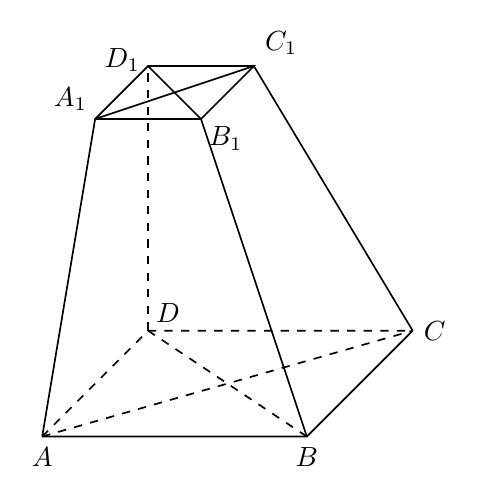
\begin{tikzpicture}[scale=1.12, semithick,
  every node/.style={inner sep=1.5pt}]
  \coordinate (A)  at (0,0);
  \coordinate (B)  at (3,0);
  \coordinate (C)  at (4.2,1.2);
  \coordinate (D)  at (1.2,1.2);
  \coordinate (A1) at (0.6,3.6);
  \coordinate (B1) at (1.8,3.6);
  \coordinate (C1) at (2.4,4.2);
  \coordinate (D1) at (1.2,4.2);
  % 被遮棱与底面辅助线
  \draw[dashed] (A) -- (D) -- (C);
  \draw[dashed] (D) -- (D1);
  \draw[dashed] (A) -- (C);
  \draw[dashed] (B) -- (D);
  % 可见棱
  \draw (A) -- (B) -- (C);
  \draw (C) -- (C1);
  \draw (A) -- (A1) -- (B1) -- (B);
  \draw (B1) -- (C1) -- (D1) -- (A1);
  % 上底面对角线
  \draw (A1) -- (C1);
  \draw (B1) -- (D1);
  % 顶点标注
  \node[anchor=north] at ([yshift=-2pt]A) {$A$};
  \node[anchor=north] at ([yshift=-2pt]B) {$B$};
  \node[anchor=west]  at ([xshift=2pt]C) {$C$};
  \node[anchor=south west] at ([xshift=1pt,yshift=1pt]D) {$D$};
  \node[anchor=south east] at ([xshift=-1pt,yshift=1pt]A1) {$A_1$};
  \node[anchor=north west] at ([xshift=1pt,yshift=-1pt]B1) {$B_1$};
  \node[anchor=south west] at ([xshift=2pt,yshift=2pt]C1) {$C_1$};
  \node[anchor=east] at ([xshift=-1pt,yshift=2pt]D1) {$D_1$};
\end{tikzpicture}
\end{center}
\nopagebreak[4]
（1）求证：$A_1C_1$ 与 $AC$ 共面，$B_1D_1$ 与 $BD$ 共面；

（2）求证：平面 $A_1ACC_1\perp$ 平面 $B_1BDD_1$；

（3）求二面角 $A-BB_1-C$ 的大小。（用反三角函数值表示）

\end{question}
\begin{question}
\gkti{18}设 $F$ 是抛物线 $G:x^2=4y$ 的焦点。

（1）过点 $P(0,-4)$ 作抛物线 $G$ 的切线，求切线方程；

（2）设 $A,B$ 为抛物线 $G$ 上异于原点的两点，且满足 $\overrightarrow{FA}\cdot\overrightarrow{FB}=0$，延长 $AF,BF$ 分别交抛物线 $G$ 于点 $C,D$，求四边形 $ABCD$ 面积的最小值。

\end{question}
\begin{question}
\gkti{19}在医学生物学试验中，经常以果蝇作为试验对象，一个关有 $6$ 只果蝇的笼子里，不慎混入了两只苍蝇（此时笼内共有 $8$ 只蝇子：$6$ 只果蝇和 $2$ 只苍蝇），只好把笼子打开一个小孔，让蝇子一只一只地往外飞，直到两只苍蝇都飞出，再关闭小孔。

（1）求笼内恰好剩下 $1$ 只果蝇的概率；

（2）求笼内至少剩下 $5$ 只果蝇的概率。

\end{question}
\begin{question}
\gkti{20}设函数 $f(x)=-\cos^2x-4t\sin\dfrac x2\cos\dfrac x2+4t^3+t^2-3t+4$，$x\in\mathbf R$，其中 $|t|\leqslant1$。将 $f(x)$ 的最小值记为 $g(t)$。

（1）求 $g(t)$ 的表达式；

（2）讨论 $g(t)$ 在区间 $(-1,1)$ 内的单调性并求极值。

\end{question}
\begin{question}
\gkti{21}某国采用养老储备金制度。公民在就业的第一年就交纳养老储备金，数目为 $a_1$，以后每年交纳的数目均比上一年增加 $d$（$d>0$），因此，历年所交纳的储备金数目 $a_1,a_2,\cdots$ 是一个公差为 $d$ 的等差数列。与此同时，国家给予优惠的计息政策，不仅采用固定利率，而且计算复利。这就是说，如果固定年利率为 $r$（$r>0$），那么，在第 $n$ 年末，第一年所交纳的储备金就变为 $a_1(1+r)^{n-1}$，第二年所交纳的储备金就变为 $a_2(1+r)^{n-2}$，$\cdots$。以 $T_n$ 表示到第 $n$ 年末所累计的储备金总额。

（1）写出 $T_n$ 与 $T_{n-1}$（$n\geqslant2$）的递推关系式；

（2）求证：$T_n=A_n+B_n$，其中 $\{A_n\}$ 是一个等比数列，$\{B_n\}$ 是一个等差数列。

\end{question}